% Insert these two subsections within the existing appendix section
% Routing and fusion: protocols and supplementary results.
% Remove their old versions from experimental_diagnostics.tex to avoid
% duplicate labels. Keep the Circular internal-routing subsection there.
% Uses the existing bm, amsmath, booktabs, and graphicx packages and PDFs.

\subsection{Output-space fusion: conditional algebraic identities}
\label{app:fusion_consistency}

We first derive how fixed-weight fusion affects constraints, residuals,
and energy, then compare the candidates and their blend using common
diagnostic operators in Appendix~\ref{app:fusion_measured}. The identities
separate inherited candidate properties from additional fusion terms;
their empirical consequences must be evaluated rather than assumed.

\paragraph{Assumptions and linear constraints.}
Let $\bm u_\alpha=\alpha\bm u_1+\beta\bm u_2$ and
$p_\alpha=\alpha p_1+\beta p_2$, where $\beta=1-\alpha$,
$\alpha\in[0,1]$ is constant in space and time within each prediction
window, and both candidates share a mesh, parameter, time grid, and
pressure gauge. For a common linear operator $D_h$,
$D_h\bm u_\alpha=\alpha D_h\bm u_1+\beta D_h\bm u_2$.
Consequently, zero discrete divergence, a zero-mean pressure gauge,
and identical affine boundary constraints are preserved if both
candidates satisfy them. This conditional statement does not establish
that the learned candidate fields satisfy these constraints.

\paragraph{Nonlinear residuals.}
For a fixed bilinear discretization $N_h$, define
$\delta\bm u=\bm u_1-\bm u_2$. Then
\begin{equation}
N_h(\bm u_\alpha,\bm u_\alpha)
=\alpha N_h(\bm u_1,\bm u_1)+\beta N_h(\bm u_2,\bm u_2)
-\alpha\beta N_h(\delta\bm u,\delta\bm u).
\end{equation}
Using the sign convention
$R_u(\bm u,p)=\partial_t\bm u-\bm f_h-L_h\bm u
+N_h(\bm u,\bm u)+G_hp$, this yields
\begin{equation}
R_u(\bm u_\alpha,p_\alpha)
=\alpha R_u(\bm u_1,p_1)+\beta R_u(\bm u_2,p_2)
-\alpha\beta N_h(\delta\bm u,\delta\bm u).
\end{equation}
Similarly, for
$R_p(\bm u,p)=A_hp-[\bm s_0+S_1\bm u+B_p(\bm u,\bm u)]$
with fixed bilinear $B_p$,
\begin{equation}
R_p(\bm u_\alpha,p_\alpha)
=\alpha R_p(\bm u_1,p_1)+\beta R_p(\bm u_2,p_2)
+\alpha\beta B_p(\delta\bm u,\delta\bm u).
\end{equation}
The additional terms separate the fusion defect from the candidates'
existing residuals; they need not increase or decrease the residual
norm. These are algebraic identities under the stated assumptions,
not evaluations of the native CFD equations. State-dependent limiters
or other non-bilinear discretizations require their actual operators.

\paragraph{Kinetic energy.}
For $E(\bm u)=\tfrac12\|\bm u\|_M^2$ with a common positive
quadrature matrix $M$,
\begin{equation}
E(\bm u_\alpha)=\alpha E(\bm u_1)+\beta E(\bm u_2)
-\frac{\alpha\beta}{2}\|\bm u_1-\bm u_2\|_M^2.
\end{equation}
Thus candidate disagreement reduces the blend's energy relative to the
weighted candidate energies, potentially including phase cancellation.
It does not imply lower energy than both candidates or improved agreement
with the reference. The blend is not fed back into either specialist,
so this term is not a recurrent dissipative modification of their dynamics.

\subsection{Square: measured physical-field diagnostics}
\label{app:fusion_measured}

\paragraph{Evaluation set and comparison fields.}
We evaluate both candidates, their frozen T2-C blend, and a common
POD-reconstructed reference on the same 16 held-out windows per Square
interface used for fusion evaluation ($K=24$, output spacing 4).
The candidates are Steady/Hopf for S--H and Periodic/Hopf for H--P.
Each interface contains two parameter values with eight overlapping
windows each. No window is selected by prediction quality, and overlapping
windows are not treated as independent experimental replications.
These measurements concern reconstructed fields, not errors against
unprojected CFD fields or residuals of the original OpenFOAM discretization.

\paragraph{Spatial operators and temporal differences.}
On the common 9,400-cell grid, quadratic local least-squares fits define
$D_x,D_y$, and the Laplacian $L$. The initial stencil contains 24 nearest
cells with independent coordinate scaling; it is expanded only if the
polynomial matrix is rank-deficient or its condition number exceeds
$10^6$. A second version starts from 36 neighbors to test sensitivity;
actual stencils contain at most 72 cells. Both versions differentiate
a manufactured quadratic polynomial with maximum absolute error below
$1.4\times10^{-10}$. This check verifies polynomial reproduction, not
accuracy on all reconstructed flow fields. We compute
\begin{align}
\widehat R_u&=\delta_t\bm u+N_D(\bm u,\bm u)
+\nabla_Dp-\mathrm{Re}^{-1}L\bm u,\\
\widehat R_p&=Lp+D_xN_{D,x}+D_yN_{D,y},
\end{align}
where $N_D(\bm u,\bm u)=uD_x\bm u+vD_y\bm u$ and
$N_{D,x},N_{D,y}$ are its two components. Centered temporal differences
and summary statistics use output steps 2--23.

\paragraph{Metrics and averaging.}
Residuals are summarized by area-weighted RMS over the interior wake
$6\leq x\leq16$, $1\leq y\leq3$ (2,627 cells). For a scalar or vector
residual $r$, this is
\begin{equation}
\|r\|_{\mathrm{RMS},\Omega_w}
=\left(\frac{\sum_{i\in\Omega_w}w_i\|r_i\|_2^2}
{\sum_{i\in\Omega_w}w_i}\right)^{1/2}.
\end{equation}
Kinetic energy uses quadrature over the whole domain. We distinguish
the energy error from the candidate-relative fusion deficit:
\begin{align}
\varepsilon_E&=100\frac{|E(\bm u)-E_{\rm ref}|}{E_{\rm ref}},\\
d_E&=100\frac{\alpha E(\bm u_1)+\beta E(\bm u_2)
-E(\bm u_\alpha)}{E_{\rm ref}},
\end{align}
where $E_{\rm ref}=E(\bm u_{\rm ref})$. Both quantities are percentages,
but only $\varepsilon_E$ measures agreement with reference energy.
Statistics average the evaluated steps and windows within each parameter,
then weight the two parameters equally.

\begin{table}[tbp]
\centering\small
\caption{Square physical-field diagnostics with the 24-neighbor initial
stencil. Energy error is evaluated over the whole domain; residuals are
interior area-weighted RMS, not percentages. Entries average output steps
2--23 and the evaluation windows as described above. Reference denotes
POD-reconstructed CFD rather than raw CFD.}
\label{tab:fusion_residual_measured}
\begin{tabular}{@{}llrrr@{}}
\toprule
Interface & Field & Energy error (\%) & $\|\widehat R_u\|$ & $\|\widehat R_p\|$\\
\midrule
S--H & Reference & 0 & 0.00460 & 0.03395\\
& Steady & 2.81100 & 0.00530 & 0.03674\\
& Hopf & 0.14296 & 0.00607 & 0.03513\\
& T2-C & 0.17641 & 0.00520 & 0.03421\\
\midrule
H--P & Reference & 0 & 0.11486 & 0.03736\\
& Periodic & 0.09163 & 0.11627 & 0.03785\\
& Hopf & 0.17298 & 0.11189 & 0.04047\\
& T2-C & 0.05974 & 0.11408 & 0.03631\\
\bottomrule
\end{tabular}
\end{table}

\paragraph{Measured comparisons and interpretation.}
Table~\ref{tab:fusion_residual_measured} shows different outcomes for
different diagnostics. On S--H, T2-C has smaller momentum and pressure
residuals than either candidate, but Hopf has a smaller energy error.
On H--P, T2-C has the smallest pressure residual and energy error among
the predictions, whereas Hopf has the smallest momentum residual.
The pressure-residual ordering also holds with the 36-neighbor initial
stencil, although changing the stencil changes residual magnitudes
substantially. The reference residual is nonzero and includes POD
truncation and spatial/temporal differentiation error; it is not a solver
convergence tolerance. In particular, a predicted field can have a lower
diagnostic residual than the reference without being more accurate.

\paragraph{Additional effects of fusion.}
As an implementation check, the conditional identities agree to within
$6.1\times10^{-14}$ across both stencils and all windows.
Figure~\ref{fig:fusion_energy_defects_supp} isolates fusion-induced
changes from the total errors in Table~\ref{tab:fusion_residual_measured}.
Besides $d_E$, we report the RMS of the additional residual fields
\begin{equation}
\Delta\widehat R_q
=\widehat R_q(\bm u_\alpha,p_\alpha)
-\alpha\widehat R_q(\bm u_1,p_1)
-\beta\widehat R_q(\bm u_2,p_2),
\qquad q\in\{u,p\}.
\end{equation}
The norm is taken after subtracting the residual fields; it is not
a difference between residual norms.

The mean normalized energy deficit $d_E$ is $0.00314\%$ for S--H and
$0.00181\%$ for H--P over steps 2--23. Thus the average energy reduction
relative to the weighted candidate energies is small on these windows;
this is not a bound on individual-window deviations or the error
against reference energy. The curves show that the additional residuals
are nonzero and time-dependent: S--H exhibits an early peak and a
secondary rise, whereas H--P shows a later increase.
Their magnitudes alone do not determine whether the total fused
residual improves, because the additional fields interact with the
candidates' existing residuals. These results characterize the finite
evaluation windows, not long-time stability or strict conservation.

\begin{figure}[tbp]
\centering
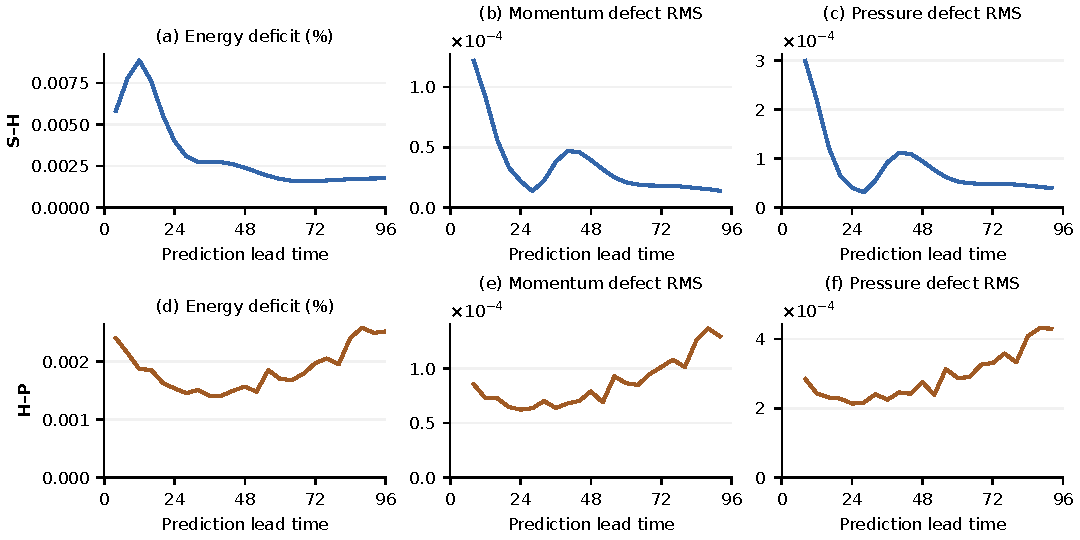
\includegraphics[width=\linewidth]{figures/fusion_defects_compact.pdf}
\caption{Additional effects of Square T2-C fusion with the 24-neighbor
initial stencil. Rows correspond to S--H (top) and H--P (bottom);
columns show normalized energy deficit $d_E$ in percent, momentum-defect
RMS, and pressure-defect RMS. Each curve averages all 16 windows at each
prediction lead time. Energy uses steps 1--24; residuals use steps 2--23.
Residual RMS is computed over the interior wake before window averaging.
The energy deficit is relative to weighted candidate energies, not
reference-energy error; residual defects are not total residuals.
Axes use panel-specific scales.}
\label{fig:fusion_energy_defects_supp}
\end{figure}
